\chapter{Entrepreneurial Judgment: Mindset, Scale, and Learned Risk}

In this interview Lavon Perrin presents entrepreneurship less as inspiration than as a sequence of judgments. We are asked to watch how a person interprets circumstance, chooses peers, allocates evening hours, sets a target, tests whether work is scalable, and learns from mistakes without freezing. The mathematics here is modest and largely reconstructive, but it is still useful: a few simple comparisons, update rules, and arithmetic examples carry much of the lecture's practical force.

\section{Social Environment as an Opening Claim}

The lecture opens before the formal interview begins. Instead of a definition, we are given a proverb: if one spends time with nine broke friends, one becomes the tenth; if one spends time with nine people driving Ferraris, one's odds improve. The point is not to prove a sociological theorem. The point is to plant a strong heuristic: environment acts on us continuously, and it acts before we notice it.

We can write that opening claim in the deliberately rough form suggested by the transcript:
\begin{align}
n_{\text{broke}} &= 9 \Rightarrow \text{self} \to \text{10th broke peer},\\
n_{\text{ambitious}} &= 9 \Rightarrow P(\text{upward move}) \uparrow .
\end{align}

\begin{remark}
These relations are heuristics, not laws. Perrin is compressing a practical belief about exposure, aspiration, and behavioral drift into an arithmetic image that can be remembered.
\end{remark}

Only after this cold open does the host identify the setting and the guest. We are told that this is the first School of Hard Knocks installment of the ``10 Questions with Millionaires'' format, and the lecture then narrows immediately to the first real problem: what separates people in business?

\section{Mindset as the Primary Tool}

The first substantive answer is uncompromising. Perrin says that the main separator is mindset. In these notes it is useful to state what that means operationally. Mindset is not merely mood. It is the rule by which a situation is read, and therefore the rule by which the next action is chosen.

\begin{definition}
Mindset is the interpretive structure that sits between event and action. In Perrin's use of the term, it determines whether a given situation is read as possibility, obstruction, or excuse.
\end{definition}

A compact reconstruction is
\begin{equation}
\text{Situation} + \text{Mindset} \to \text{Interpretation} \to \text{Action}.
\end{equation}

This is why he moves so quickly from mindset to the news, negativity, and self-accountability. If the interpretive mechanism is damaged, then even an ordinary situation will be read as a negative one. The lecture is careful here: the point is not vague positivity, but control of inputs and responsibility for outputs. The news example matters because it tells us that the mind is not a sealed chamber. It is trained by what it consumes.

\subsection{Question \& Answer}

\paragraph{Question.} If mindset is really the decisive tool, where do we first see it in practice?

\paragraph{Answer.} We see it at the moment when blame is turned inward and then converted into action. Perrin asks, in effect, why one is not where one wants to be, and he answers by forcing the listener to look in the mirror. That shift is immediately followed by a practical example: the side hustle. So the lecture moves from psychology to arithmetic. It asks not only how we think, but what hours remain available once we stop saying that nothing can be done.

His example uses the East Coast and West Coast time difference. If calls would ordinarily stop at \(8{:}00\) p.m. in one time zone, then a West Coast market extends the reachable workday by three hours:
\begin{align}
t_{\text{close,East}} &= 20{:}00,\\
\Delta t &= 3\ \text{hours},\\
t_{\text{close,West}} &= t_{\text{close,East}} + \Delta t = 23{:}00.
\end{align}

The transcript gives a worked entrepreneurial example rather than a general slogan:
\paragraph{Worked example.}
\begin{enumerate}
\item Hold the primary job during the day.
\item Have dinner and attend family obligations.
\item Return home at \(20{:}00\).
\item Call into a West Coast market until \(23{:}00\).
\item Repeat until the secondary stream is large enough to replace the first job.
\end{enumerate}

The mechanism can be summarized by a narrow vertical reconstruction:

\begin{figure}[h]
\centering
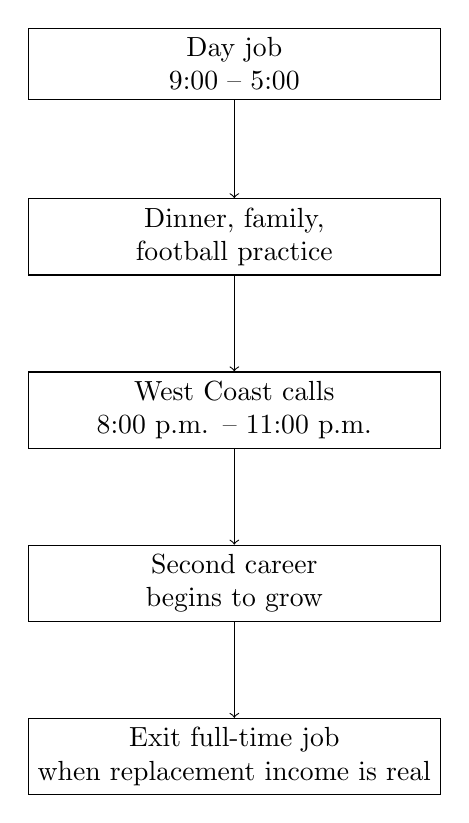
\begin{tikzpicture}
\node[draw, rectangle, text width=5.0cm, align=center] (a) at (0,0) {Day job\\\(9{:}00\) -- \(5{:}00\)};
\node[draw, rectangle, text width=5.0cm, align=center] (b) at (0,-2.2) {Dinner, family,\\football practice};
\node[draw, rectangle, text width=5.0cm, align=center] (c) at (0,-4.4) {West Coast calls\\\(8{:}00\) p.m. -- \(11{:}00\) p.m.};
\node[draw, rectangle, text width=5.0cm, align=center] (d) at (0,-6.6) {Second career\\begins to grow};
\node[draw, rectangle, text width=5.0cm, align=center] (e) at (0,-8.8) {Exit full-time job\\when replacement income is real};
\draw[->] (a) -- (b);
\draw[->] (b) -- (c);
\draw[->] (c) -- (d);
\draw[->] (d) -- (e);
\end{tikzpicture}
\end{figure}

The lecture's point is not that every business should be built by cold-calling. The point is that the right mindset uncovers a convertable resource. In this case that resource is time.

\section{From Corporate Misfit to Doing One's Own Thing}

After the general advice, the interviewer asks for a turning point. The answer is important because Perrin does not narrate entrepreneurship as a single flash of revelation. He says, more cautiously, that it ``just kind of happened.'' That matters. We are not being given a myth of destiny. We are being given a slower account of mismatch, apprenticeship, and eventual independence.

Corporate America, in his telling, did not fit comfortably. He had too many questions, he bucked the system, yet he was a capable salesperson, was liked, and could lead people. That mixture is the crucial biographical fact. The same traits that produced friction inside an organization later become useful inside his own venture. So the lecture reframes previous employment not as wasted time but as training.

We can compress that biographical logic into a simple chain:
\begin{equation}
\text{Corporate work} \to \text{sales skill} + \text{leadership} + \text{business knowledge} \to \text{independent action}.
\end{equation}

That chain is immediately sharpened by a constraint. Perrin says that the car business carried a family cost he did not want, and he wanted to be able to see his children. So the entrepreneurial turn is not motivated only by money or ego. It is also shaped by a life-structure decision. One door closes, another opens, but the opening is chosen under pressure from both ambition and family life.

\section{Scaling by Planning, Replication, and Environment}

The next major question concerns scale, and here the lecture becomes more explicit about targets. Perrin argues that many people want to make \(\$100{,}000\) a year, but that this is precisely the problem: the target is too small. He then offers a striking asymmetry. If one plans for \(\$500{,}000\) and misses, one might still arrive near \(\$100{,}000\). It is not a theorem; it is a motivational asymmetry designed to expose the weakness of low targets.

\subsection{Question \& Answer}

\paragraph{Question.} What actually enables a business to scale?

\paragraph{Answer.} First a larger target, then a plan for reaching it, and then a test of whether the present standard of work is worth reproducing. Perrin does not speak here in the language of formal optimization, but the structure is clear: target, plan, replication, accountability, and only then environment.

The target comparison may be written as
\begin{align}
G_{\text{ordinary}} &= \$100{,}000,\\
G_{\text{stretch}} &= \$500{,}000,\\
Y_{\text{miss stretch}} &\approx \$100{,}000.
\end{align}

The mathematical content is intentionally simple. If we aim low, then even success is small. If we aim high, then even failure may land on territory that low aiming would have treated as its maximum.

Perrin's most operational idea in this section is the ``10 of me'' test.

\begin{definition}
The ``10 of me'' test asks whether ten copies of one's present standard of work would improve the firm or the client experience. If the answer is yes, the underlying behavior is not merely energetic; it is reproducible and therefore scalable.
\end{definition}

A compact reconstruction is
\begin{equation}
S = \text{Value}(10\times \text{me}) - \text{Value}(1\times \text{me}),
\qquad
S>0 \text{ indicates a scalable standard.}
\end{equation}

He then folds the opening proverb back into the scale discussion. Accountability remains central, but accountability alone is not enough. One must also choose a better environment. This is where the Ferrari line returns with a fuller meaning. It is not merely about luxury. It is about placing oneself near people who normalize a different level of action, income, and lifestyle.

So the section closes on a reconstructed rule:
\begin{equation}
\text{Better peer set} \to P(\text{desired conduct and outcome}) \uparrow .
\end{equation}

The move downtown is offered as a concrete example of that rule. He wanted to be around people already doing the kinds of things he wanted to do. In the lecture's own rhythm, the teaser has now become an argument.

\section{Risk, Sales, and Personal Development}

Once growth has been discussed, the next question is unavoidable: what does growth cost? Perrin's answer is direct. There is no success without risk. The listener is not allowed to imagine a perfectly safe path to unusual outcomes.

But the risk here is not theatrical risk. It is calculated risk. It must be joined to self-belief, education, and the willingness to learn from outcomes. The lecture's practical update rule can be written as
\begin{equation}
\text{Action} + \text{Calculated Risk} \to \text{Outcome} \to \text{Learning} \to \text{Better Next Action}.
\end{equation}

That is the right level of abstraction for this lecture. We are not given a probability model. We are given a disciplined rule for not collapsing after uncertainty has produced a result.

\subsection{Question \& Answer}

\paragraph{Question.} What is the secret to sales?

\paragraph{Answer.} Perrin gives the surprising answer that the secret is personal development. He does not begin with scripts, lines, or closing tricks. He begins with reading, study, and the long work of understanding one's own motives and ambitions.

This answer matters because it takes the earlier risk section and internalizes it. If risk is to be taken intelligently, then the person taking it must be improved. That is why he speaks about books not simply as sources of information, but as instruments that clarified why his thoughts and ambitions were already arranged as they were.

The transcript gives one concrete numerical measure:
\begin{equation}
B_{\text{last year}} \approx 15,
\qquad
B_{\text{previous year}} \ll B_{\text{last year}}.
\end{equation}

Again, this is not a universal benchmark. It is a concrete sign that self-development changed from a vague value into a repeated practice.

The books named in the lecture are:
\begin{itemize}
\item \textit{Think and Grow Rich},
\item \textit{Rich Dad Poor Dad},
\item \textit{Go for No}.
\end{itemize}

The order is important. First comes the claim that personal development matters, then comes the list of books, and only after that comes the reflective point: reading helped him validate his own tendencies, ambitions, and energies. The books matter because they change the operator, not because they furnish slogans.

\section{Owning a Business: Mistakes, Time, and Money}

The later part of the lecture descends from aspiration into operating discipline. The interviewer asks about the biggest business challenge, then about the worst financial decision, then about work-life balance, and finally about money and happiness. These are not unrelated questions. Together they form a single block about judgment under pressure.

\subsection{Question \& Answer}

\paragraph{Question.} How does an owner learn without being destroyed by mistakes?

\paragraph{Answer.} Perrin answers by insisting that ownership is repetitive adjustment. There will be ups and downs, budgeting decisions, growth decisions, and mistakes. The task is not to avoid all error. The task is to learn from error without freezing into overanalysis.

The lecture's opposition can be written simply as
\begin{align}
\text{mistake} &\to \text{lesson},\\
\text{overanalysis} &\to \text{no motion}.
\end{align}

This is the same update logic we saw earlier, now stated in a more operational setting. His BMW anecdote belongs here. The transcript is somewhat rough in detail, but the core point is clear enough: a desired purchase was not necessarily wrong in itself, yet it was handled without enough foresight about maintenance and ongoing cost. The lesson is not merely ``do not buy.'' The lesson is ``buy within a plan.''

The work-life balance answer continues the same theme. Perrin does not really offer balance as a poetic ideal. He offers leverage. He points to a figure such as the head of Amazon and remarks, in effect, that the day itself is not longer for such a person. What differs is the use of that day and the presence of people around him who can multiply output.

A compact reconstruction is
\begin{equation}
T_{\text{day,Bezos}} = T_{\text{day,us}} = 24\ \text{hours}.
\end{equation}

So the difference must come from structure, delegation, and judgment, not from a hidden reserve of time. In that spirit one may write
\begin{equation}
\text{Output} = \text{own effort} + \text{leveraged effort of others}.
\end{equation}

He begins to invoke the familiar contrast between going somewhere fast alone and going farther with others. The transcript breaks before the line is completed, but the surrounding point is clear: entrepreneurship eventually becomes a problem of coordinated effort.

The final question concerns money and happiness, and here the lecture ends soberly. Money may buy freedom if it is handled well, but it does not automatically buy happiness. The key variable is management capacity. Hence the strong comparison:
\begin{align}
\neg \text{Manage}(\$1{,}000) &\Rightarrow \neg \text{Manage}(\$1{,}000{,}000),\\
\text{Money} + \text{Judgment} &\to \text{Freedom},\\
\text{Money} &\neq \text{Happiness}.
\end{align}

This is a fitting end to the lecture. We began with environment and mindset, and we end with the same deep logic in another register. Wealth does not save a person from bad judgment. It amplifies whatever judgment is already there.

\section{Summary}

Perrin's interview is organized around entrepreneurial judgment. Mindset governs interpretation. Interpretation governs action. Time can be reclaimed and repurposed. Prior employment can serve as apprenticeship. Scale requires higher targets, a plan, and work worth reproducing. Risk must be calculated and then converted into learning. Sales begins with personal development rather than sales theater. Business ownership means budgeting, mistakes, anti-paralysis, and leverage. Money, finally, is not identical with happiness; at best, when handled well, it purchases freedom.

That is why the opening proverb matters. The lecture never leaves it behind. It only unpacks it. We become something like the people, habits, and structures around us, unless we deliberately choose otherwise.